Summary for Advanced Computer Systems
at University of Copenhagen 2021/2022.
These notes are mostly based on the lecture slides and
reading material.

\section{Fundamentals}
\paragraph{Common Problems of Systems}
\begin{itemize}
\item \textbf{Emergent Properties} \\
  properties not showing up in individual components, but
  when combining those components

\item \textbf{Propagation of Effects} \\
  what looks at first to be a small disruption or
  a local change can have effects that reach from
  one end of a system to the other

\item \textbf{Incommensurate Scaling} \\
  as a system increases in size or speed, not all parts
  of it follow the same scaling rules, so things stop
  working

\item \textbf{Trade-offs} \\
  \textit{waterbed effect}: pushing down on a problem at one point causes
  another problem to pop up somewhere else

\end{itemize}

\paragraph{System technical definition:}
A \textbf{system} is a set of interconnected components that
has an expected behavior observed at the interface with its
environment.

Divide all the things in the world into two groups:
\begin{itemize}
\item those under discussion (part of the system)
\item those that are not part \textbf{(environment)}
\item the interactions between system and its environment
  are the \textbf{interface} between the system and environment
\end{itemize}


\paragraph{Fundamentals}
\begin{itemize}
\item Abstractions: interpreters, memory, communication links
\item Modularity with clients and services (RPC)
\item Techniques for performance
\end{itemize}

\paragraph{Learning goals}
\begin{itemize}
\item Identify the fundamental abstractions in
  computer systems
\item Explain how names are used in the fundamental abstractions
\item Being able to design a top-level abstraction, based on
  lower-level abstractions
\item Discuss performance and fault-tolerance of a design
\end{itemize}

\paragraph{Central Trade-off: Abstractions, Performance, Fault-Tolerance}
\begin{figure}[ht!]
  \centering
  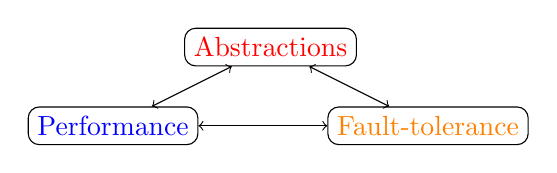
\begin{tikzpicture}
    \draw (1, 1) node
          [draw=black, rounded corners] (ab)
          {{\color{red} Abstractions}};

    \draw (-1, 0) node
          [draw=black, rounded corners] (per)
          {{\color{blue} Performance}};
    \draw (3, 0) node
          [draw=black, rounded corners] (fault)
          {{\color{orange} Fault-tolerance}};
    \draw [<->] (per) -- (fault);
    \draw [<->] (per) -- (ab);
    \draw [<->] (ab) -- (fault);
\end{tikzpicture}
\end{figure}

\paragraph{Examples for Trade-off}
\begin{itemize}
\item To improve performance one might has to ignore the abstraction
  and take the behavior of the underlying concrete implementation into
  account
\item when introducing another layer of abstraction we might
  introduce new kinds of errors (for example when introducing RPC,
  we can have communication errors)
\item introducing mechanisms for fault-tolerance can have
  a negative effect on performance
\end{itemize}

\paragraph{Names}
Names make connections between different the abstractions.

\begin{itemize}
\item Examples
  \begin{itemize}
  \item IP-address
  \item IR
  \end{itemize}
\item Names require a mapping scheme
\item How can we map names?
  \begin{itemize}
  \item Table lookup (e.g. Files inside directories)
  \item Recursive lookup
  \item Multiple lookup
  \end{itemize}
\end{itemize}

\paragraph{Memory}
\begin{itemize}
\item READ(name) $\rightarrow$ value
\item WRITE(name, value)
\end{itemize}

Examples of Memory
\begin{itemize}
\item Physical memory (RAM)
\item Multi-level memory hierarchy
\item Address spaces and virtual memory with paging
\item Key-value stores
\item Database storage engines
\end{itemize}


\paragraph{Interpreters}
Interpreter has:
\begin{itemize}
\item Instruction repertoire
\item Environment
\item Instruction pointer
\end{itemize}

Interpretation Loop:

\begin{lstlisting}
do forever
  instruction <- READ(instruction_pointer)
  perform instruction in environment context
  if interrupt_signal = True
    instruction_pointer <- entry of INTERRUPT_HANDLER
    environment <- environment of INTERRUPT_HANDLER
\end{lstlisting}

Examples of Interpreters:
\begin{itemize}
\item Processors (CPU)
\item Programming language interpreters
\item Frameworks (e.g. MapReduce, Spark)
\item layered programs (RPCs)
\end{itemize}

\paragraph{Communication links}
\begin{itemize}
\item SEND(linkName, outgoingMessageBuffer)
\item RECEIVE(linkName, incomingMessageBuffer)
\end{itemize}

Examples of Communication Links:
\begin{itemize}
\item Ethernet interface
\item IP datagram service
\item TCP sockets
\item Message-Oriented Middleware (MOM)
\item Multicast (e.g. CATOCS Causal and Totally-Ordered
  Communication System)
\end{itemize}

\paragraph{Other Abstractions}
\begin{itemize}
\item Synchronization
  \begin{itemize}
  \item Locks
  \item Condition variables \& monitors
  \end{itemize}
\item Data processing
  \begin{itemize}
  \item Data transformations
  \item Operators
  \end{itemize}
\end{itemize}

% LocalWords:  Modularity RPC MapReduce RPCs linkName datagram TCP
% LocalWords:  outgoingMessageBuffer incomingMessageBuffer Middleware
% LocalWords:  Multicast CATOCS
